\documentclass{article}
\usepackage{tikz}
\usetikzlibrary{positioning}
\usepackage[margin=0.3in, landscape]{geometry}
\pagestyle{empty}
\begin{document}

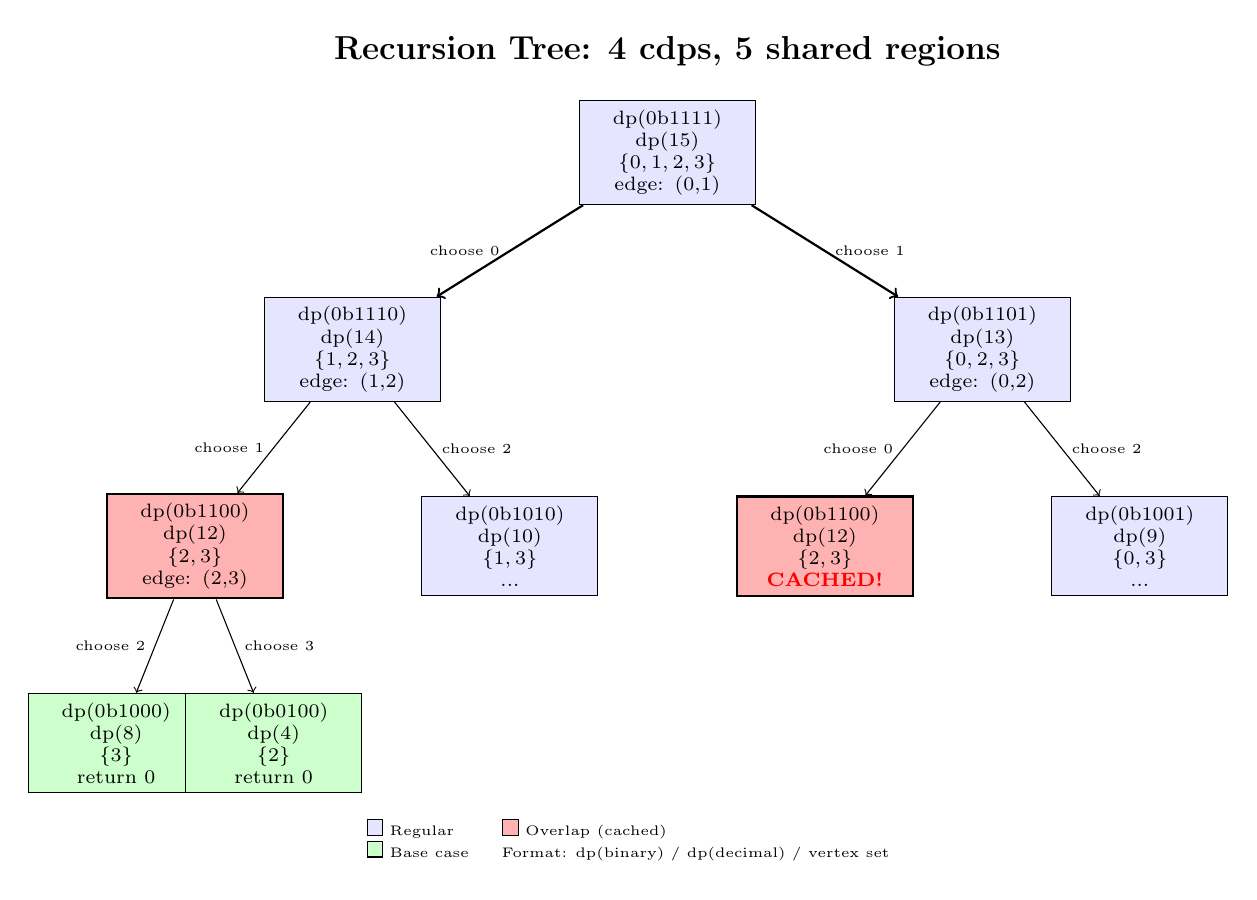
\begin{tikzpicture}[
  node/.style={rectangle, draw, fill=blue!10, minimum width=2.2cm, minimum height=1cm, font=\scriptsize, align=center, text width=2cm},
  leaf/.style={rectangle, draw, fill=green!20, minimum width=2.2cm, minimum height=1cm, font=\scriptsize, align=center, text width=2cm},
  overlap/.style={rectangle, draw, fill=red!30, minimum width=2.2cm, minimum height=1cm, font=\scriptsize, align=center, text width=2cm, thick}
]

% Level 0 (root)
\node[node] (root) at (0,0) {dp(0b1111)\\dp(15)\\$\{0,1,2,3\}$\\edge: (0,1)};

% Level 1
\node[node] (l1a) at (-4,-2.5) {dp(0b1110)\\dp(14)\\$\{1,2,3\}$\\edge: (1,2)};
\node[node] (l1b) at (4,-2.5) {dp(0b1101)\\dp(13)\\$\{0,2,3\}$\\edge: (0,2)};

% Level 2 (from l1a)
\node[overlap] (l2a1) at (-6,-5) {dp(0b1100)\\dp(12)\\$\{2,3\}$\\edge: (2,3)};
\node[node] (l2a2) at (-2,-5) {dp(0b1010)\\dp(10)\\$\{1,3\}$\\...};

% Level 2 (from l1b)
\node[overlap] (l2b1) at (2,-5) {dp(0b1100)\\dp(12)\\$\{2,3\}$\\\textcolor{red}{\textbf{CACHED!}}};
\node[node] (l2b2) at (6,-5) {dp(0b1001)\\dp(9)\\$\{0,3\}$\\...};

% Level 3 (from l2a1)
\node[leaf] (l3a1) at (-7,-7.5) {dp(0b1000)\\dp(8)\\$\{3\}$\\return 0};
\node[leaf] (l3a2) at (-5,-7.5) {dp(0b0100)\\dp(4)\\$\{2\}$\\return 0};

% Edges
\draw[->, thick] (root) -- node[left, font=\tiny] {choose 0} (l1a);
\draw[->, thick] (root) -- node[right, font=\tiny] {choose 1} (l1b);

\draw[->] (l1a) -- node[left, font=\tiny] {choose 1} (l2a1);
\draw[->] (l1a) -- node[right, font=\tiny] {choose 2} (l2a2);

\draw[->] (l1b) -- node[left, font=\tiny] {choose 0} (l2b1);
\draw[->] (l1b) -- node[right, font=\tiny] {choose 2} (l2b2);

\draw[->] (l2a1) -- node[left, font=\tiny] {choose 2} (l3a1);
\draw[->] (l2a1) -- node[right, font=\tiny] {choose 3} (l3a2);

% Title
\node[above=0.3cm of root, font=\large\bfseries] 
  {Recursion Tree: 4 cdps, 5 shared regions};

% Legend
\node[below=0.2cm of current bounding box.south, anchor=north, font=\tiny] {
  \begin{tabular}{ll}
    \tikz\node[fill=blue!10, draw, minimum size=0.2cm] {}; Regular & 
    \tikz\node[fill=red!30, draw, minimum size=0.2cm] {}; Overlap (cached) \\
    \tikz\node[fill=green!20, draw, minimum size=0.2cm] {}; Base case & 
    Format: dp(binary) / dp(decimal) / vertex set
  \end{tabular}
};

\end{tikzpicture}

\end{document}

